\documentclass{beamer}
\usetheme[pageofpages=of,% String used between the current page and the
                         % total page count.
          bullet=circle,% Use circles instead of squares for bullets.
          titleline=true,% Show a line below the frame title.
          alternativetitlepage=true,% Use the fancy title page.
       %   titlepagelogo=logo-polito,% Logo for the first page.
       %   watermark=watermark-polito,% Watermark used in every page.
       %   watermarkheight=100px,% Height of the watermark.
       %   watermarkheightmult=4,% The watermark image is 4 times bigger
                                % than watermarkheight.
          ]{Torino}

\setbeamertemplate{footline}{
  \begin{beamercolorbox}[wd=\paperwidth,ht=1ex,dp=1ex]{footline}
    \vspace{5pt} \hspace{1em} \insertframenumber/\inserttotalframenumber
  \end{beamercolorbox}
}

\author{Brendon J. Brewer}
\title{STATS 331 -- Introduction to Bayesian Statistics}
\institute{The University of Auckland}
\date{}


\linespread{1.3}
\usepackage{minted}
\usepackage[utf8]{inputenc}
\usepackage{dsfont}
\newcommand{\given}{\,|\,}
\newcommand{\balpha}{\boldsymbol{\alpha}}
\newcommand{\bmu}{\boldsymbol{\mu}}


\begin{document}

\frame{\titlepage}

\begin{frame}
\Large

\begin{center}
Review
\end{center}
\end{frame}

\begin{frame}
\frametitle{Lecture Purpose}

We will now briefly review the course content, and I will outline my
expectations for what you should be able to do in the exam.

\end{frame}


\begin{frame}
\frametitle{Probabilities}
The mathematics of {\bf probabilities} can be used to describe two different
things: proportions, and uncertainties. Which interpretation you adopt
determines the way you end up using the maths.\pause

   \begin{columns} % Create two columns

        \column{0.5\textwidth} % Left column (50% width)
        \centering
        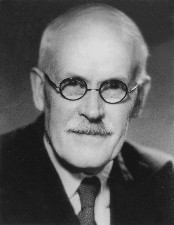
\includegraphics[width=0.5\linewidth]{images/jeffreys.jpg}

        Harold Jeffreys (Bayesian)

        \column{0.5\textwidth} % Right column (50% width)
        \centering
        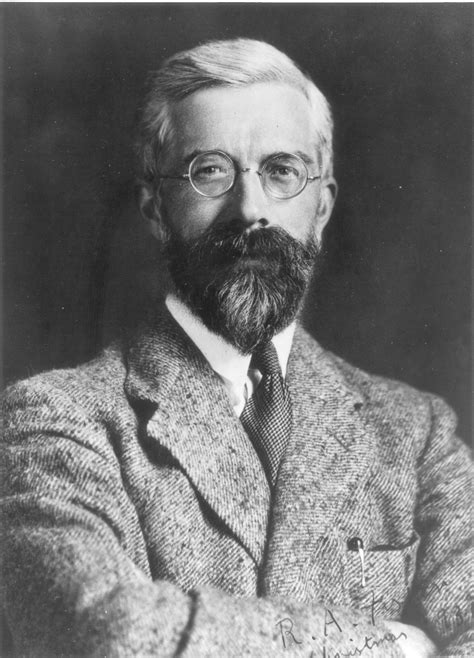
\includegraphics[width=0.5\linewidth]{images/fisher.jpg}

        R. A. Fisher (Frequentist)
     \end{columns}


\end{frame}


\end{document}

